\documentclass{article}
\usepackage{amsmath}   % For math symbols and align environment
\usepackage{amssymb}   % For additional symbols
\usepackage{graphicx}  % For including figures

\begin{document}

\section*{A4}

\subsection*{(b)}

\textbf{Cross-Entropy Loss:} Figure~\ref{fig:ce_loss} shows the training and validation loss curves for all models trained with the cross-entropy loss function.

\begin{figure}[ht]
    \centering
    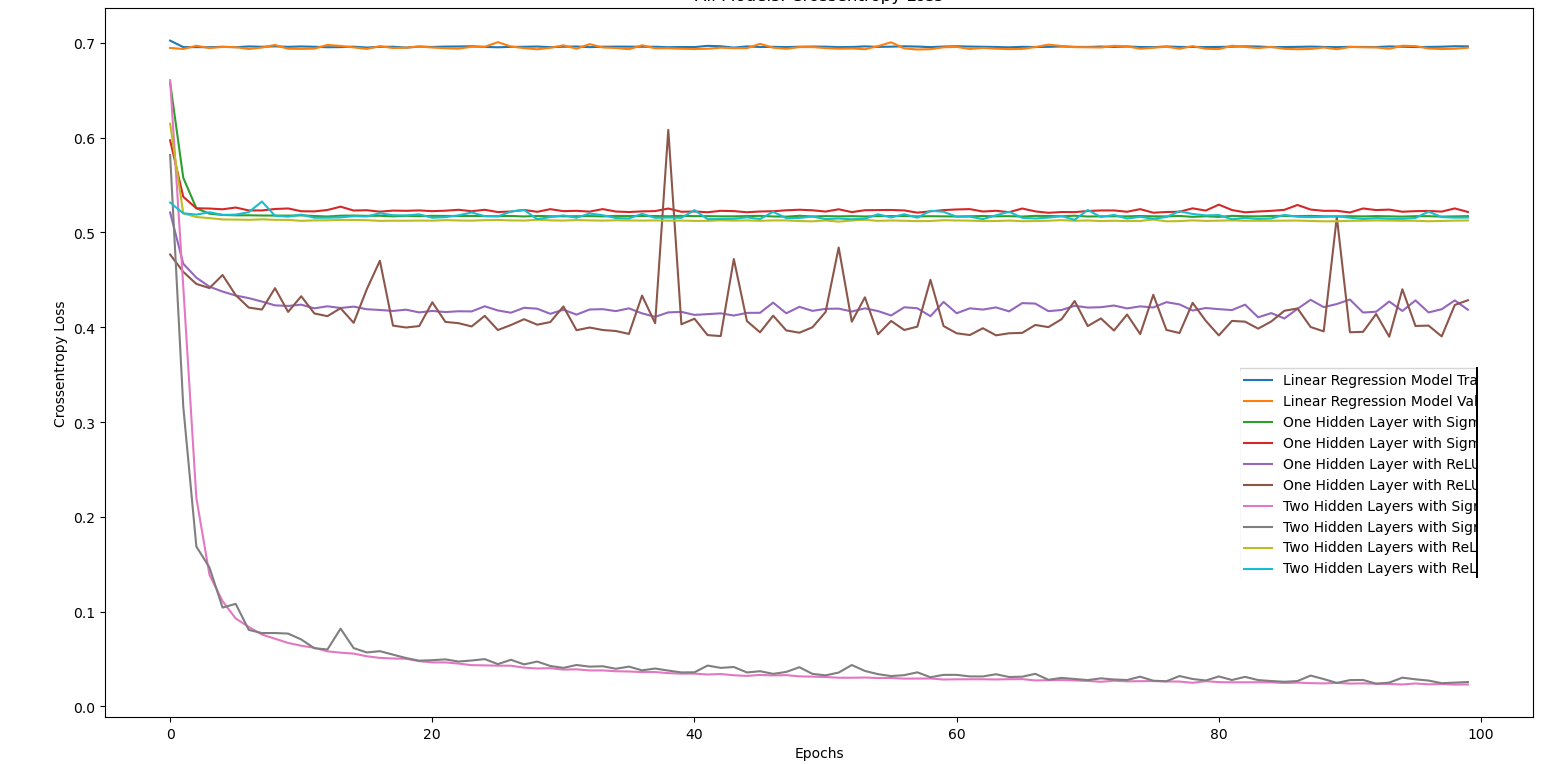
\includegraphics[width=0.7\linewidth]{cross_entropy_loss.png}
    \caption{Training and Validation Loss Curves for All Models (Cross-Entropy Loss).}
    \label{fig:ce_loss}
\end{figure}

\textbf{MSE Loss:} Figure~\ref{fig:mse_loss} shows the training and validation loss curves for all models trained with the MSE loss function.

\begin{figure}[ht]
    \centering
    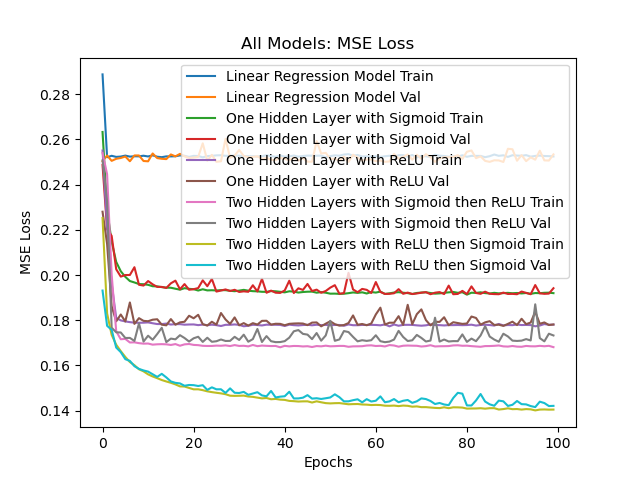
\includegraphics[width=0.7\linewidth]{mse_loss.png}
    \caption{Training and Validation Loss Curves for All Models (MSE Loss).}
    \label{fig:mse_loss}
\end{figure}

\subsection*{(c)}

\textbf{Cross-Entropy Loss:}  
The best model trained with cross-entropy loss was a network with two hidden layers using Sigmoid then ReLU activation functions. It achieved a test set accuracy of \(0.9928\). The scatter plot of its predictions is shown in Figure~\ref{fig:ce_scatter}.

\begin{figure}[ht]
    \centering
    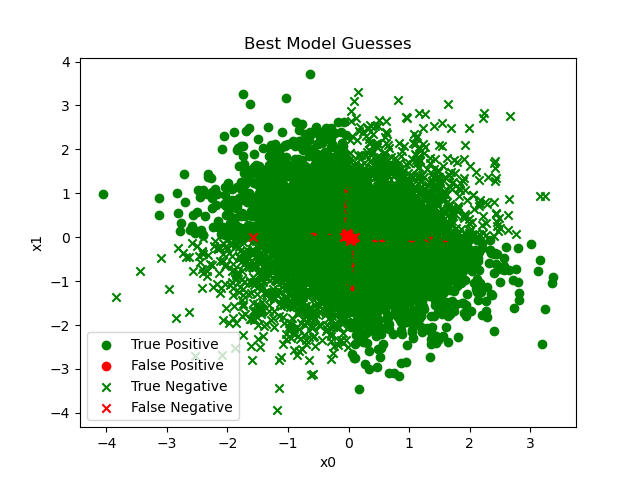
\includegraphics[width=0.7\linewidth]{cross_entropy_scatter.png}
    \caption{Scatter Plot of Best Cross-Entropy Model (Two Hidden Layers with Sigmoid then ReLU).}
    \label{fig:ce_scatter}
\end{figure}

\textbf{MSE Loss:}  
The best model trained with MSE loss was a network with two hidden layers using ReLU then Sigmoid activation functions. It achieved a test set accuracy of \(0.7212\). The scatter plot of its predictions is shown in Figure~\ref{fig:mse_scatter}.

\begin{figure}[ht]
    \centering
    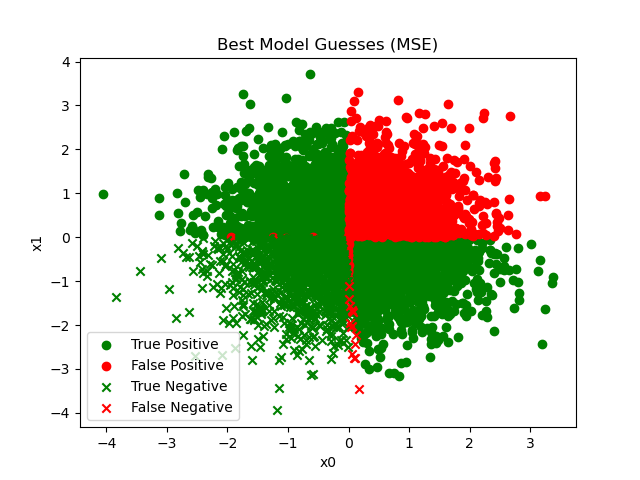
\includegraphics[width=0.7\linewidth]{mse_scatter.png}
    \caption{Scatter Plot of Best MSE Model (Two Hidden Layers with ReLU then Sigmoid).}
    \label{fig:mse_scatter}
\end{figure}

\end{document}
